\begin{quote}
    \textit{``This [tidal force divergence] is related to something that happens in AdS/CFT. \ldots don't tell anyone I mentioned that.'' --Jorge Santos}
\end{quote}

Quick announcement-- office hours from this course will be held at 14:00 on Tuesdays. If you plan to attend the office hours, however, do send an email in advance.

Last time, we started looking at the geodesics of Schwarzschild. We found two particularly simple ones: the ingoing and outgoing radial null geodesics, with equation
\begin{equation}
    \frac{dt}{dr} = \pm \paren{1-\frac{2M}{r}
    }^{-1}, \quad r> 2M.
\end{equation}
We also defined the tortoise (Regge-Wheeler) coordinate $r_*$ such that
\begin{equation}
    dr_* =\frac{dr}{1-\frac{2M}{r}}.
\end{equation}
Thus our null geodesic equation becomes
\begin{equation}
    \frac{dt}{dr_*}=\pm 1.
\end{equation}
In tortoise coordinates, null geodesics therefore obey
\begin{equation}
    t=\pm r_* + \text{constant}.
\end{equation}
This seems kind of trivial. But now we introduce a new coordinate, the \term{ingoing Eddington-Finkelstein coordinate}, defining
\begin{equation}
    v \equiv t+ r_*.
\end{equation}
This is clearly constant on ingoing geodesics, just by looking at the previous equation. That is, $dv=dt+dr_*=0.$ Good.%
    \footnote{We could have done the same for outgoing geodesics taking $u\equiv t-r_*,$ and indeed we will do so later.} 
Now we eliminate the original coordinate time $t$ from the line element using $dt=dv-\frac{dr}{1-\frac{2M}{r}}.$ We get the new line element
\begin{equation}
    ds^2 = -\paren{1-\frac{2M}{r}} dv^2 +2dv dr +r^2 d\Omega^2_2.
\end{equation}
%black holes are type D solutions
Let's write this in matrix notation. Nothing fancy.
\begin{equation}
    g_{\mu\nu}=\begin{pmatrix}
        -\paren{1-\frac{2M}{r}} & 1 & 0 & 0\\
        1 & 0 & 0 & 0\\
        0 & 0 & r^2 & 0\\
        0 & 0 & 0 & r^2\sin^2\theta
    \end{pmatrix}.
\end{equation}
We haven't done anything too extreme, just made a change of coordinates. But we see something very nice-- none of the metric components are singular at $r=2M$. In fact, the determinant of the metric is still perfectly nice at $r=2M$-- by an explicit computation, $\det g= -r^4 \sin^2 \theta$. This only vanishes at $\theta=0$, which is the regular coordinate badness%
    \footnote{AKA degeneracy. Basically, what is the value of $\phi$ at the north pole? It's not well-defined, hence our coordinates do not define an invertible map from coordinates to manifold points.}
of spherical coordinates near the poles, and at $r=0$, which may be a real problem (a priori, we don't know yet).

So we have found some coordinates which appear to extend $r$ not just from $r>2M$ but to all $r>0$. Our metric is real and analytic (i.e. we've shown the determinant is nonsingular) so it is a nice analytic continuation of the old (bad) Schwarzschild coordinates. This is related to the problem of \term{extendibility}-- are there other metrics which cover more of the spacetime manifold which are compatible with the solution that we've found?

However, something really bad does happen as $r\to 0$. The Kretchmann scalar $R^{abcd}R_{abcd}=\frac{48 M^2}{r^6} \to \infty$ as $r\to 0$, and scalars by definition are invariant under coordinate transformations. So we cannot get rid of this by a simple redefinition of coordinates.
%This [tidal force divergence] is related to something that happens in AdS/CFT. ...don't tell anyone I mentioned that.

Moreover, let us observe that %$\P{}{t}=\P{}{v}$. Thus 
our Killing vector field becomes
\begin{equation}
    K=\P{}{t} = \P{x^\mu}{t}\P{}{x^\mu}=\P{}{v} \implies K^2=g_{vv} =-\paren{1-\frac{2M}{r}}.
\end{equation}
So our metric appears to be no longer static or stationary in these coordinates.

We now introduce the Finkelstein diagram, shown in Figure \ref{fig:reall_finkelsteindiagram}. Recall that for $r=2M$, on outgoing geodesics we have $t-r_*={}$constant $\implies v= 2r+4 M \log \abs*{\frac{r}{2M}-1}+$constant. Let us draw a plot in the $t_* \equiv v-r,r$ plane. What we see is that the ingoing geodesics follow 45${}^\circ$ paths, while the outgoing geodesics follow some curved paths in these coordinates. %copy picture from Harvey Reall notes

\begin{figure}
    \centering
    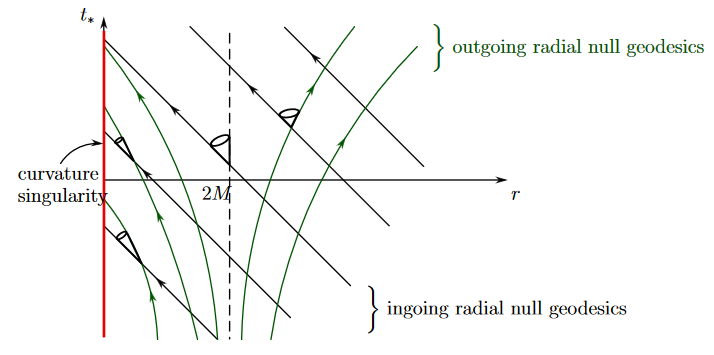
\includegraphics[width=0.8\textwidth]{2019/01/20190124_reall_finkelsteindiagram.png}
    \caption{
    The Finkelstein diagram for the Schwarzschild spacetime. The sides of the light cones are given by lines of constant $u$ and $v$. Notice the light cones ``tip over'' as we cross the event horizon at $r=2M$, so that even ``outgoing'' radial null trajectories must proceed towards the $r=0$ singularity.
    \newline
    Image credit to Prof. Reall's  \href{http://www.damtp.cam.ac.uk/user/hsr1000/black_holes_lectures_2016.pdf}{Black Holes notes}, \textsection 2.5.
    }
    \label{fig:reall_finkelsteindiagram}
\end{figure}

In these coordinates, the light cones ``tip over'' at $r=2M$-- even the ``outgoing'' null geodesics are forced to proceed towards $r=0$ for $r<2M$. Now, this does not yet prove that this is a black hole. We've only examined radial geodesic trajectories, and it's not clear that adding even a little bit of angular momentum can't save us from a spaghettified death by black hole.%(-like object).
    \footnote{Strictly, death by ``black hole-like object'' at this point, in the same sense that the Higgs boson was first reported as a ``Higgs-like particle.'' That is to say, out of an abundance of caution.}

Suppose that we%
    \footnote{``Imagine that you, not me, are situated at the surface of this star. I don't want to go there.'' -- Jorge Santos
    }
sit on the surface of a collapsing star. What we can show is that the time to singularity is $\Delta t = \mathbb{T} M$, where $M=M_\odot \implies \Delta t= \SI{10e-5}{\second}.$ It's a weird fact that we can indeed cross the horizon and hit the singularity in finite time, and yet because the event horizon is a surface of infinite redshift, a far-away observer will never see us actually cross the event horizon.
%Pictures are nice, but they can be very deceiving. ...try to go to a dating site.

\subsection*{Black hole region} 
How do we define a black hole? Before we can do that, we'll need some preliminaries.
\begin{defn} 
    A vector is \term{causal} if it is null or timelike and nonzero. A curve is causal if its tangent vector is everywhere causal.
\end{defn}
\begin{defn}
    A spacetime is \term{time-orientable} if it admits a time orientation, i.e. a causal vector field $T^a$. Another causal vector field $x^a$ is then \term{future-directed} if it lies in the same light cone as $T^a$ (i.e. $x^a T_a \leq 0$) and is past-directed otherwise.
\end{defn}
Note that the old coordinate time $t$ in Schwarzschild turned out to be a bad choice inside the event horizon. This is because $\P{}{t}$ becomes spacelike inside the horizon, related to the change of sign of $g_{tt}$ for $r<2M$.
So let us instead take $\pm \P{}{r}$, and note that in our EF coordinates, $g_{rr}=0$. Therefore $\P{}{r}\P{}{r}=0$, meaning that we've found a vector field which is null everywhere.

In fact, recall that our timelike Killing vector $K$ gave us a good sense of a time direction outside. We see that
\begin{equation*}
    K \cdot \paren{-\P{}{r}} =-g_{vr} = -1,
\end{equation*}
where $K\equiv \P{}{v}$. This tells us that $-\P{}{r}$ and $K$ lie in the same light cone, so we've found a null (hence causal) vector field which is good everywhere and defines a good time orientation for $r>0$.

\begin{prop}
Let $x^\mu(\lambda)$ be any future-directed causal curve, i.e. one whose tangent vector is everywhere future-directed and causal. Assume $r(\lambda_0)\leq 2M$ in the Schwarzschild spacetime. Then $r(\lambda)\leq 2M$ for any $\lambda \geq \lambda_0.$
\end{prop}

Let us define the tangent vector $V^\mu = \frac{dx^\mu}{d\lambda}$. Since $V^a$ is future-directed, we have %$\paren{-\P{}{r}}$ and $V^a$ are both future-directed, we have
\begin{equation}
    0\geq \paren{-\P{}{r}} V = -g_{r\mu} V^\mu = -V^v = -\frac{dv}{d\lambda} \implies \frac{dv}{d\lambda} \geq 0.
\end{equation}
Now
\begin{equation}
    V^2 \equiv V^a V_a = -\paren{1-\frac{2M}{r}}\paren{\frac{dv}{d\lambda}}^2 +2\paren{\frac{dv}{d\lambda}} \paren{\frac{dr}{d\lambda}}+r^2 \paren{\frac{d\Omega}{d\lambda}}^2,
\end{equation}
where $\paren{\frac{d\Omega}{d\lambda}}^2 \equiv \paren{\frac{d\theta}{d\lambda}}^2 +\sin^2 \theta \paren{\frac{d\phi}{d\lambda}}^2.$
Then
\begin{equation}\label{dvdlambdacondition}
    -2\paren{\frac{dv}{d\lambda}}\paren{\frac{dr}{d\lambda}}=-V^2 +\paren{\frac{2M}{r}-1} \paren{\frac{dv}{d\lambda}}^2 + r^2 \paren{\frac{d\Omega}{d\lambda}}^2.
\end{equation}
But if $V$ is causal and $r\leq 2M,$ then the right side of \ref{dvdlambdacondition} is non-negative, so it follows that
\begin{equation}
    \frac{dv}{d\lambda}\frac{dr}{d\lambda} \leq 0.
\end{equation}
Let us assume that $\frac{dr}{d\lambda}>0$ (our curve at any point is directed towards larger $r$). Then $\frac{dv}{d\lambda}=0$, which means that by \ref{dvdlambdacondition}, $V^2=0$ and $\frac{d\Omega}{d\lambda}=0$. But then the only nonvanishing component of $V$ is $V^r=\frac{dr}{d\lambda} >0 \implies V$ is a positive multiple of $\P{}{r}$, and hence is past-directed.%
    %\footnote{You might wonder how this squares with the calculation that $\paren{-\P{}{r}}V =-g_{r\mu}V^\mu.$ It seems like we should just get $-g_{rr}$, which is zero in EF coordinates. The subtlety is that $\pm\P{}{r}$ is null in these coordinates, whereas it was either spacelike or timelike in Schwarzschild depending on where we sit (inside or outside the event horizon). If we changed back to Schwarzschild, we would have $-g_{rr}>0$ and we could see that 
    %}
We have reached a contradiction.

Therefore $\frac{dr}{d\lambda}\leq 0$ if $r\leq 2M$. If $r< 2M$, the equality must be strict. If $\frac{dr}{d\lambda}=0$ then by \ref{dvdlambdacondition}, $\frac{d\Omega}{d\lambda}=\frac{dv}{d\lambda}=0 \implies V^\mu=0$. Hence if $r(\lambda_0) < 2M$, then $r(\lambda)$ is monotonically decreasing for all $\lambda \geq \lambda_0$.